\chapter{Prototipo}
Una vez creado el núcleo de la aplicación, para llevarlo al usuario final se debe encapsular en dos capas: \Gls{interfaz} y \gls{framework}. La primera capa es totalmente visual, lo que el usuario va a ver y con lo que va a interactuar, por eso es tan importante contar con una \gls{interfaz} sencilla e intuitiva que permita a cualquier persona entender como utilizar la aplicación. La segunda capa se puede definir como el pegamento que une la \gls{interfaz} con la funcionalidad para encontrar recetas, gestiona las llamadas al núcleo y da formato a la \gls{interfaz} que ve el usuario.

\section{Interfaz}
En el apartado de \textit{\gls{design}} se detallaba la interfaz de baja fidelidad para el prototipo, esta se ha llevado a cabo como una primera versión de interfaz para conocer las opiniones de los usuarios y poder mejorarla de cara al futuro.
 
\subsection{Diseño}
Siguiendo los \gls{mockup} presentados de la aplicación web, se intenta realizar en mayor medida una \gls{interfaz} sencilla que una persona mayor pueda entender, si el diseño está muy recargado es muy probable que se confunda. En la versión final de la aplicación se puede añadir un banner que actúe como footer con anuncios, que no entorpezcan la visualización o la experiencia del usuario.

\begin{figure}[h!]
\centering
\fbox{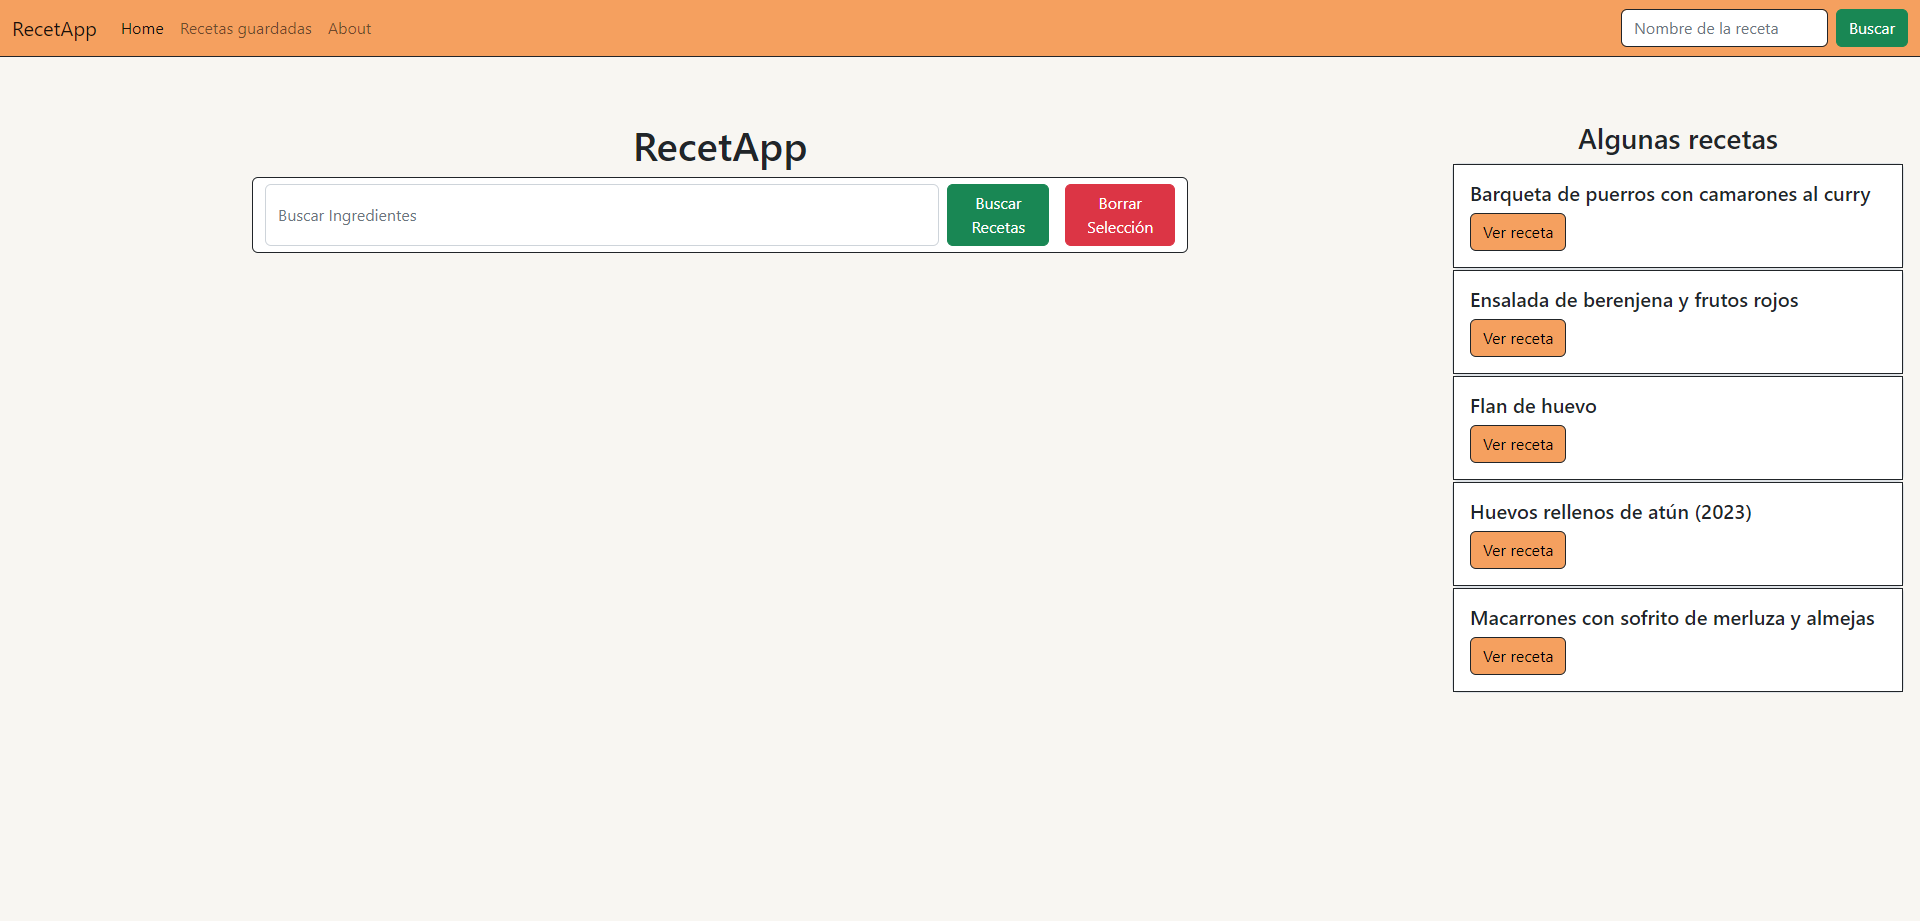
\includegraphics[width=100mm,scale=1]{./doc/imagenes/home_escritorio.png}}
\caption{Diseño para escritorio}
\label{fig:escritorio}
\end{figure}
En la figura superior se presenta la\gls{interfaz} con un diseño para escritorio. Se utiliza una barra superior a modo de navegador de la página web, con un botón para volver a la página principal y un buscador que permite buscar recetas por nombre. 

En cuanto al diseño central de la aplicación, se puede observar una clara división en dos zonas. El buscador de recetas por ingredientes y una columna a la derecha con algunas recetas aleatorias para inspirar al usuario, estas irán cambiando mientras el usuario utiliza la aplicación. Los resultados del buscador aparecerán bajo la barra de búsqueda.
\newpage
\begin{figure}[h!]
\centering
\fbox{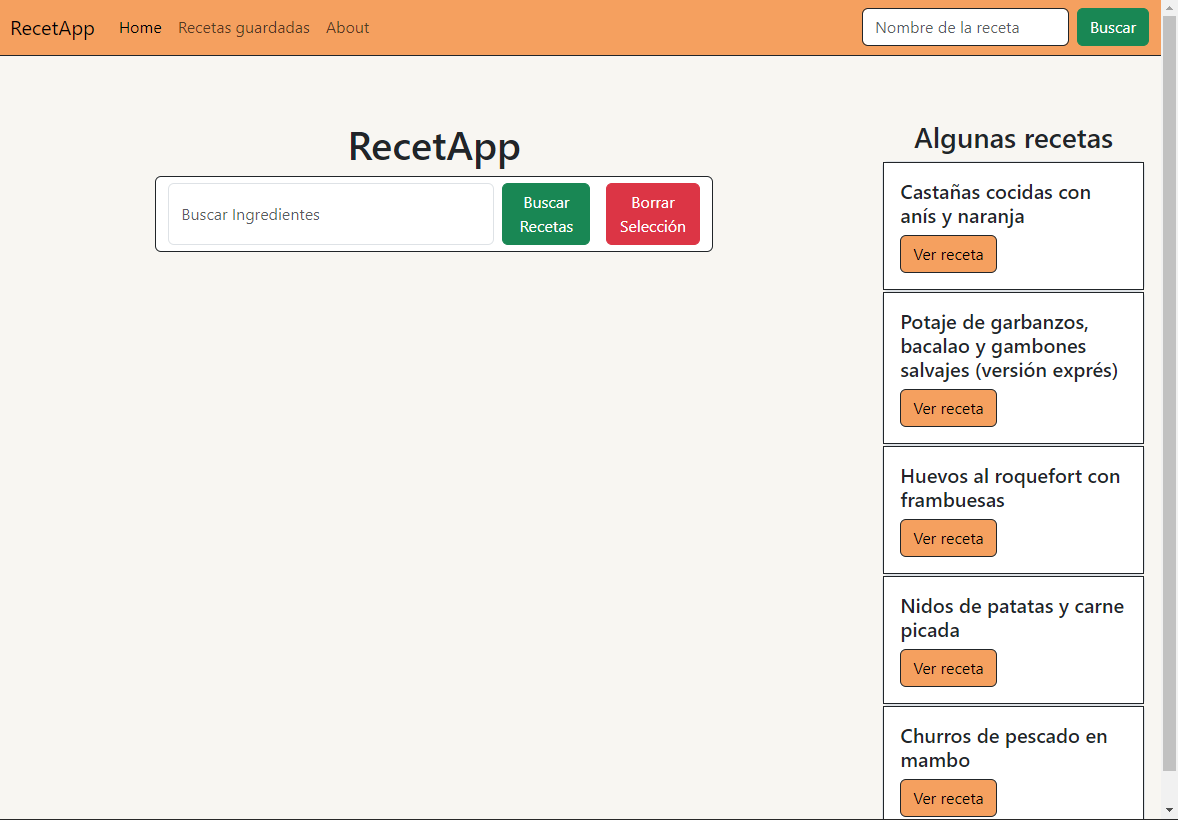
\includegraphics[width=100mm,scale=1]{./doc/imagenes/home_ipad_horizontal.png}}
\caption{Diseño para tableta horizontal}
\label{fig:surface}
\end{figure}
La figura superior muestra un diseño para una tableta en modo horizontal, siendo muy parecida al diseño de escritorio, excepto el navegador que colapsaría mostrando el botón para desplegarlo y la desaparición del cuadro que explicaría el uso del buscador.

\begin{figure}[b!p]
\centering
\fbox{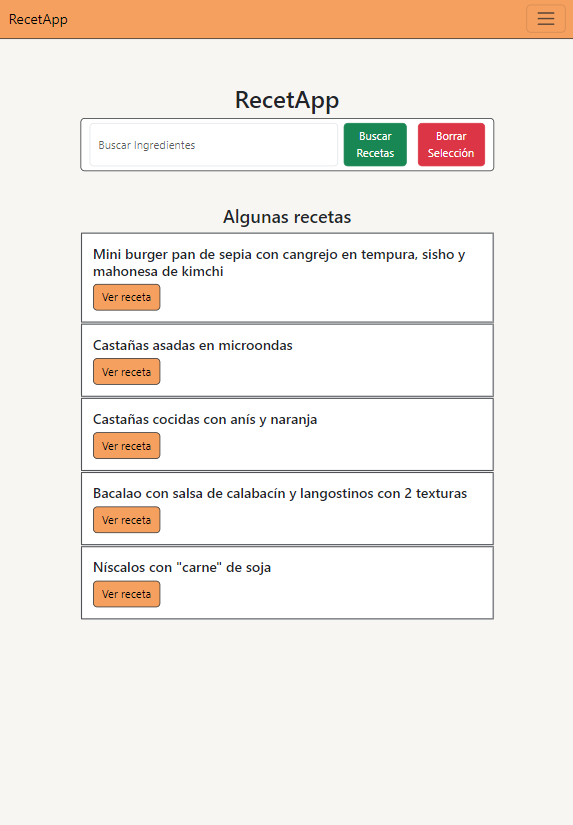
\includegraphics[width=85mm,scale=1]{./doc/imagenes/home_vertical.png}}
\caption{Diseño para tableta vertical}
\label{fig:ipad}
\end{figure}
Por último, se muestra el diseño para una tableta vertical más estrecha. Se puede observar que la zona central que antes estaba dividida en dos, se ha pasado a una sola columna con el objetivo de que los resultados sean lo más legibles posible. Este mismo diseño es el utilizado para dispositivos móviles.

\subsection{Implementación}
Para la parte de implementación de la interfaz se ha utilizado \href{https://getbootstrap.com/}{Boostrap}, un \emph{\gls{framework}} de estilos orientado a la facilitar una mejora visual al código \gls{HTML} sin tener que entrar a \gls{CSS} (Cascade Style Sheet). Existen otros \glspl{framework} de estilo, pero Boostrap es muy completo, no solo incluyendo estilos \gls{CSS} sino también algunas funcionalidades en JavaScript, para mejorar la interfaz, haciéndola dinámica.

Para instalar el \gls{framework}, existen dos maneras diferentes:
\begin{itemize}
    \item Descargar el código fuente
    \item Utilizar un Content Delivery Network (\gls{CDN})
\end{itemize}

Para incluirlo en el proyecto se debe añadir el \gls{tag} ``link'' con la referencia al fichero descargado o el enlace al \gls{CDN}. Por otra parte Boostrap usa elementos dinámicos que necesitan de unas funciones escritas en JavaScript incluidas en el mismo fichero comprimido descargable, que será necesario incluir dentro de un \gls{tag} ``script'', una vez añadidos los ficheros necesarios, el estilo se puede aplicar añadiendo clases a los elementos \gls{HTML}, como se haría con un \gls{CSS} normal.

El buscador principal contiene una tabla en principio oculta, esperando a ser utilizado. Cuando se escribe una letra, se empieza a buscar el resultado de la cadena en la base de datos, y los resultados se escriben dinámicamente en una tabla para que el usuario pueda seleccionar el ingrediente que desea usar. Esta función se realiza con \gls{JQuery}, usando un evento \textit{input} en el campo de búsqueda. Cada vez que se desencadena el evento se genera, con \gls{AJAX}, una petición a un \gls{endpoint} de la aplicación web, que devuelve una lista de ingredientes coincidentes.
\begin{figure}[h!]
\centering
\fbox{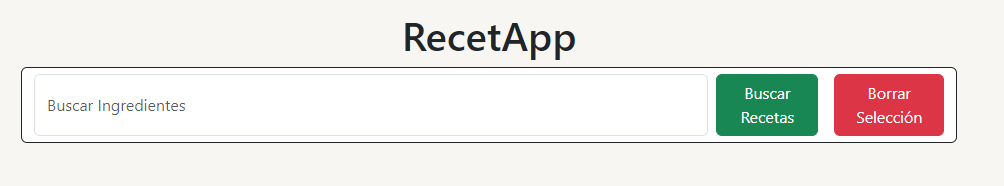
\includegraphics[width=123mm,scale=1]{./doc/imagenes/buscador.png}}
\label{fig:buscador}
\begin{lstlisting}[style=consola]
    <div class="d-inline-flex w-100">
        <input id="buscador-ingredientes" class="form-control me-2" type="search" placeholder="Buscar Ingredientes" aria-label="Search">
        <button id="enviarIngredientes" class="btn btn-success" type="submit">Buscar Recetas</button>
    <div id="eliminarSeleccion" class="btn btn-danger ms-3">Borrar Seleccion</div>
\end{lstlisting}
\caption{Diseño del buscador}
\end{figure}

La función que recupera los ingredientes de la base de datos se ha codificado en JavaScript y es llamada cada vez que el \gls{endpoint} devuelve una lista de ingredientes encontrados, es la función que da forma a la tabla de manera dinámica. \textit{buscarIngrediente} obtiene como parámetro la respuesta con la lista de ingredientes. En primer lugar, se crea la \gls{cookie} que contendrá la lista de ingredientes seleccionados. Y se elimina el atributo \textit{hidden}, para que se visualicen los resultados. Posteriormente por cada ingrediente de la lista se crea una nueva fila a la que se le añaden los atributos del ingrediente recuperado, y un disparador de eventos que al pulsar la fila añade el identificador del ingrediente a la lista almacenada en la \gls{cookie} mencionada. Si se selecciona el elemento, se muestra un \textit{tick} que permite al usuario conocer si cuenta con ese ingrediente en su lista, al volver a seleccionar el ingrediente se elimina de la ``despensa'' del usuario y se vuelve a esconder el \textit{tick}.
\begin{figure}[h!]
\centering
\fbox{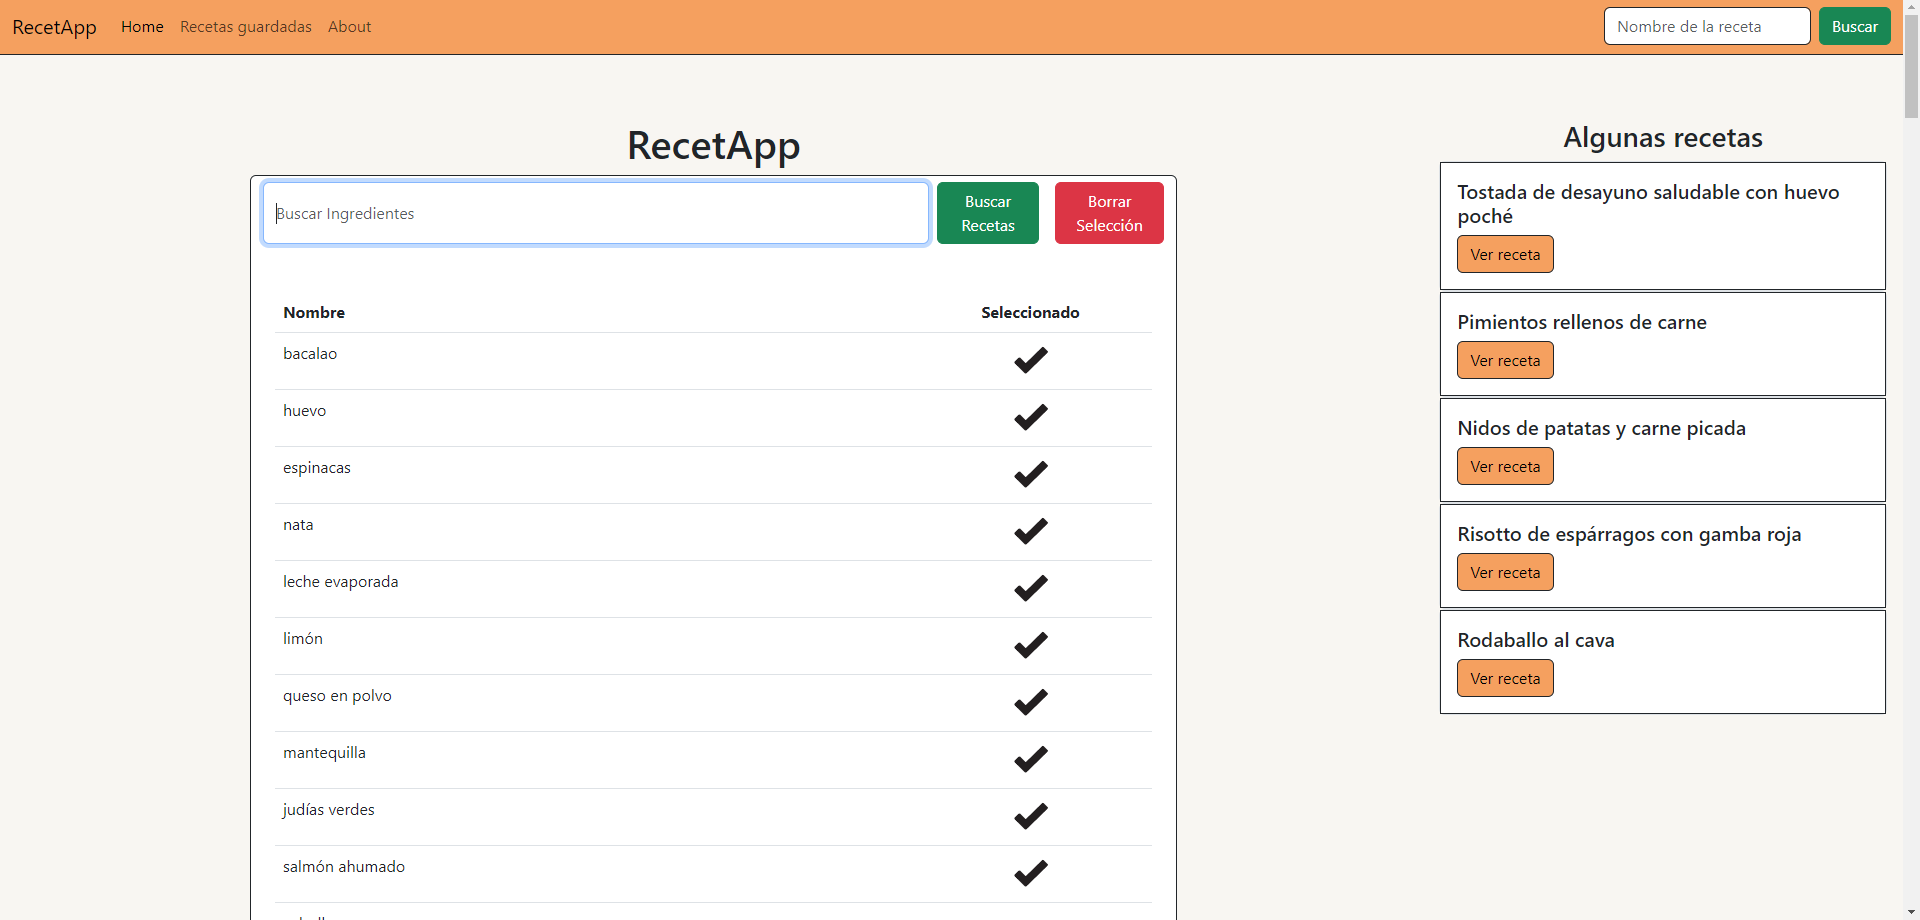
\includegraphics[width=125mm,scale=1]{./doc/imagenes/buscador_tabla.png}}
\label{fig:buscador-tabla}
\begin{lstlisting}[style=consola]
    <table id="tabla" class="table mt-5 container ingredientes">
        <thead>
            <tr>
                <th>Nombre</th>
                <th class="text-center">Seleccionado</th>
            </tr>
        </thead>
        <tbody id="tabla-ingredientes" class="">
            <tr data-id="6" onclick="SeleccionarIngrediente(this)">
                <td>canela</td>
                <td>especias</td>
                <td class="text-center">
                    <svg hidden=""></svg>
                </td>
            </tr>
        </tbody>
    </table>
\end{lstlisting}
\caption{Diseño del buscador con resultados}
\end{figure}

Por simplicidad se ha añadido solo el código \gls{HTML} relativo a una sola entrada de ingrediente. En este, como se mencionaba anteriormente, se puede observar como cada fila de la tabla cuenta con un atributo \textit{data-id}, que contiene el identificador del ingrediente. Cuando es seleccionado, se llama a la función \textit{SeleccionarIngrediente} con la fila seleccionada como argumento. Cabe destacar que no es el único método de añadir un disparador de eventos a un elemento. 

\begin{figure}[H]
    \begin{lstlisting}[style=consola]
         var resultados = response.resultados;
            tabla.empty();
            for (var i = 0; i < resultados.length; i++) {
                var fila = $('<tr data-id="'+resultados[i].id+'" onclick="SeleccionarIngrediente(this)">');
                fila.append($('<td>').text(resultados[i].nombre));
                var td = $('<td class="text-center">');
                var svg = '<svg';
                if(isSeleccionado(resultados[i].id) == false){
                    svg += " hidden"
                }
                svg += '<codigo del svg>'
                td.append(svg);
                fila.append(td);
                tabla.append(fila);
            }
\end{lstlisting}
\caption{Añadir ingredientes a la interfaz del buscador}
\label{sni:JSBuscar}
\end{figure}

\textit{SeleccionarIngrediente} selecciona el elemento \gls{SVG} (Scalable Vector Graphics) de la fila con el ingrediente seleccionado, y lo muestra. Además, obtiene la \gls{cookie} donde se almacena la lista de elementos seleccionados por el usuario y añade el identificador. El principal problema es que JavaScript almacena las \glspl{cookie} como una sola cadena de texto con un separador, es decir, antes de poder usar la lista hay que obtener el trozo de cadena que pertenece a dicha \gls{cookie}, haciendo una función que permita darle el formato correcto.

Los dos botones del buscador tienen la utilidad de eliminar ingredientes seleccionados y buscar recetas, como su propio nombre indica. El primero limpia la lista de ingredientes, eliminando toda la selección que ha realizado el usuario permitiéndole cambiar de parecer en los ingredientes sin tener que buscarlos uno a uno. El segundo botón manda los ingredientes al \gls{backend} para hacer la búsqueda de recetas utilizando dichos ingredientes, la gestión se explicará en la siguiente sección.

\begin{figure}[h!]
\centering
\fbox{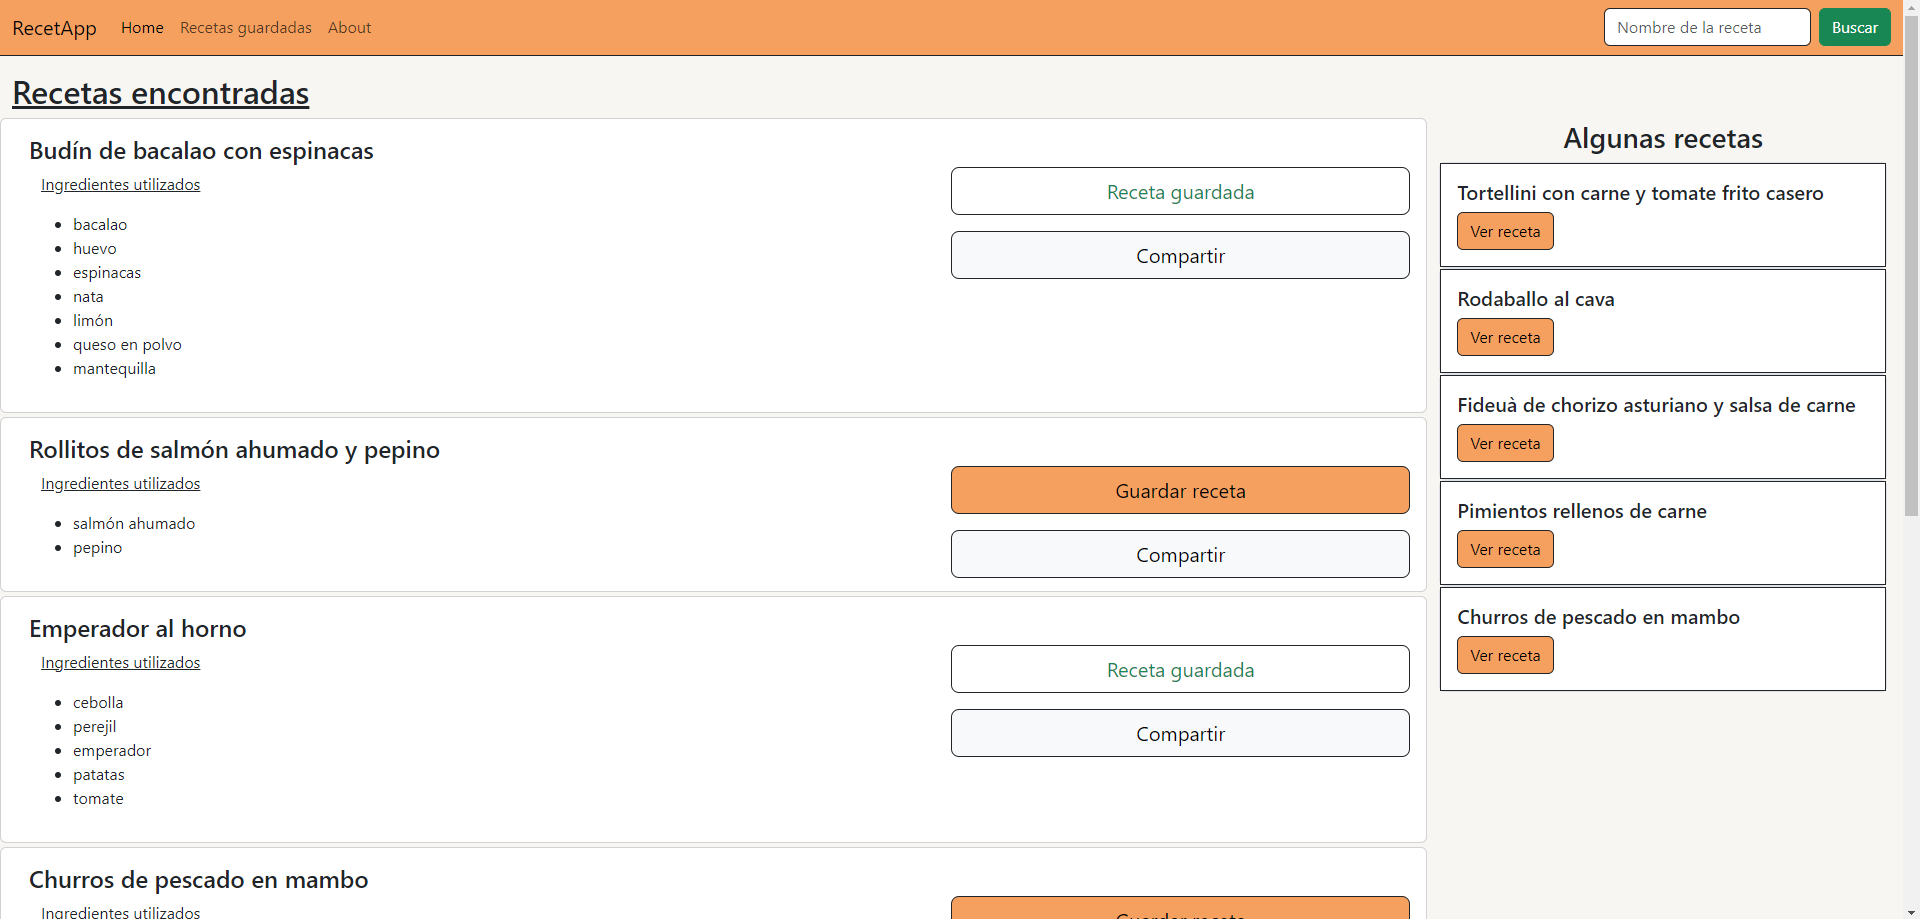
\includegraphics[width=120mm,scale=1]{./doc/imagenes/resultados_guardadas.png}}
\caption{Resultados del filtrado por ingrediente}
\label{fig:resultados}
\end{figure}

\begin{figure}[h!]
\centering
\fbox{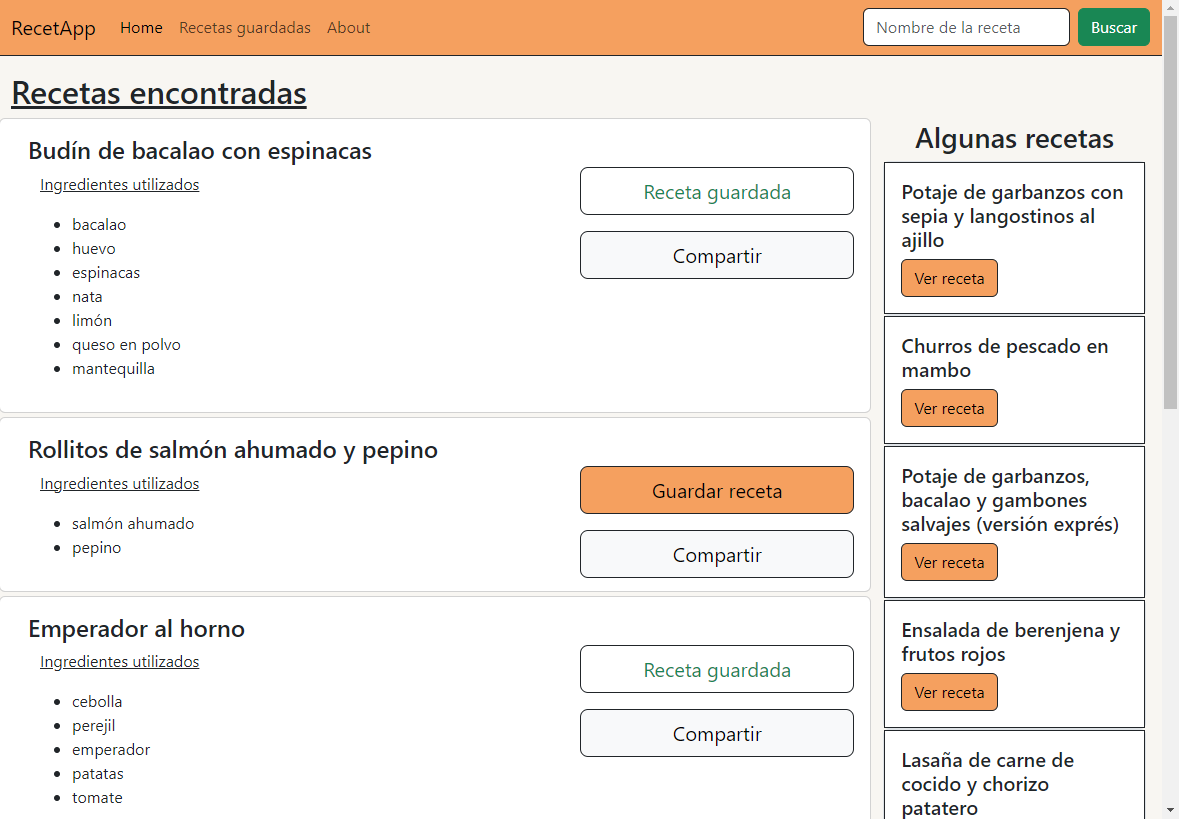
\includegraphics[width=100mm,scale=1]{imagenes/resultados_ipad.png}}
\caption{Resultados del filtrado por ingrediente en una tablet}
\label{fig:resultados-tablet}
\end{figure}

\newpage
Esta \gls{interfaz} es muy clara, ya que solo muestra recetas que se pueden realizar con los ingredientes proporcionados. Se obtiene el identificador de la receta, los nombres y sus ingredientes, para luego formatearlos en una columna de tarjetas agradable al usuario. Al seleccionar una tarjeta concreta se recupera toda la información relativa a la receta y se muestra de manera organizada. Cabe destacar que en la página de la receta no se ha añadido la columna de recetas aleatorias para enfocar la atención en la propia tarjeta de la receta, además de añadir información nutricional estimada por ración.

\begin{figure}[h!]
\centering
\fbox{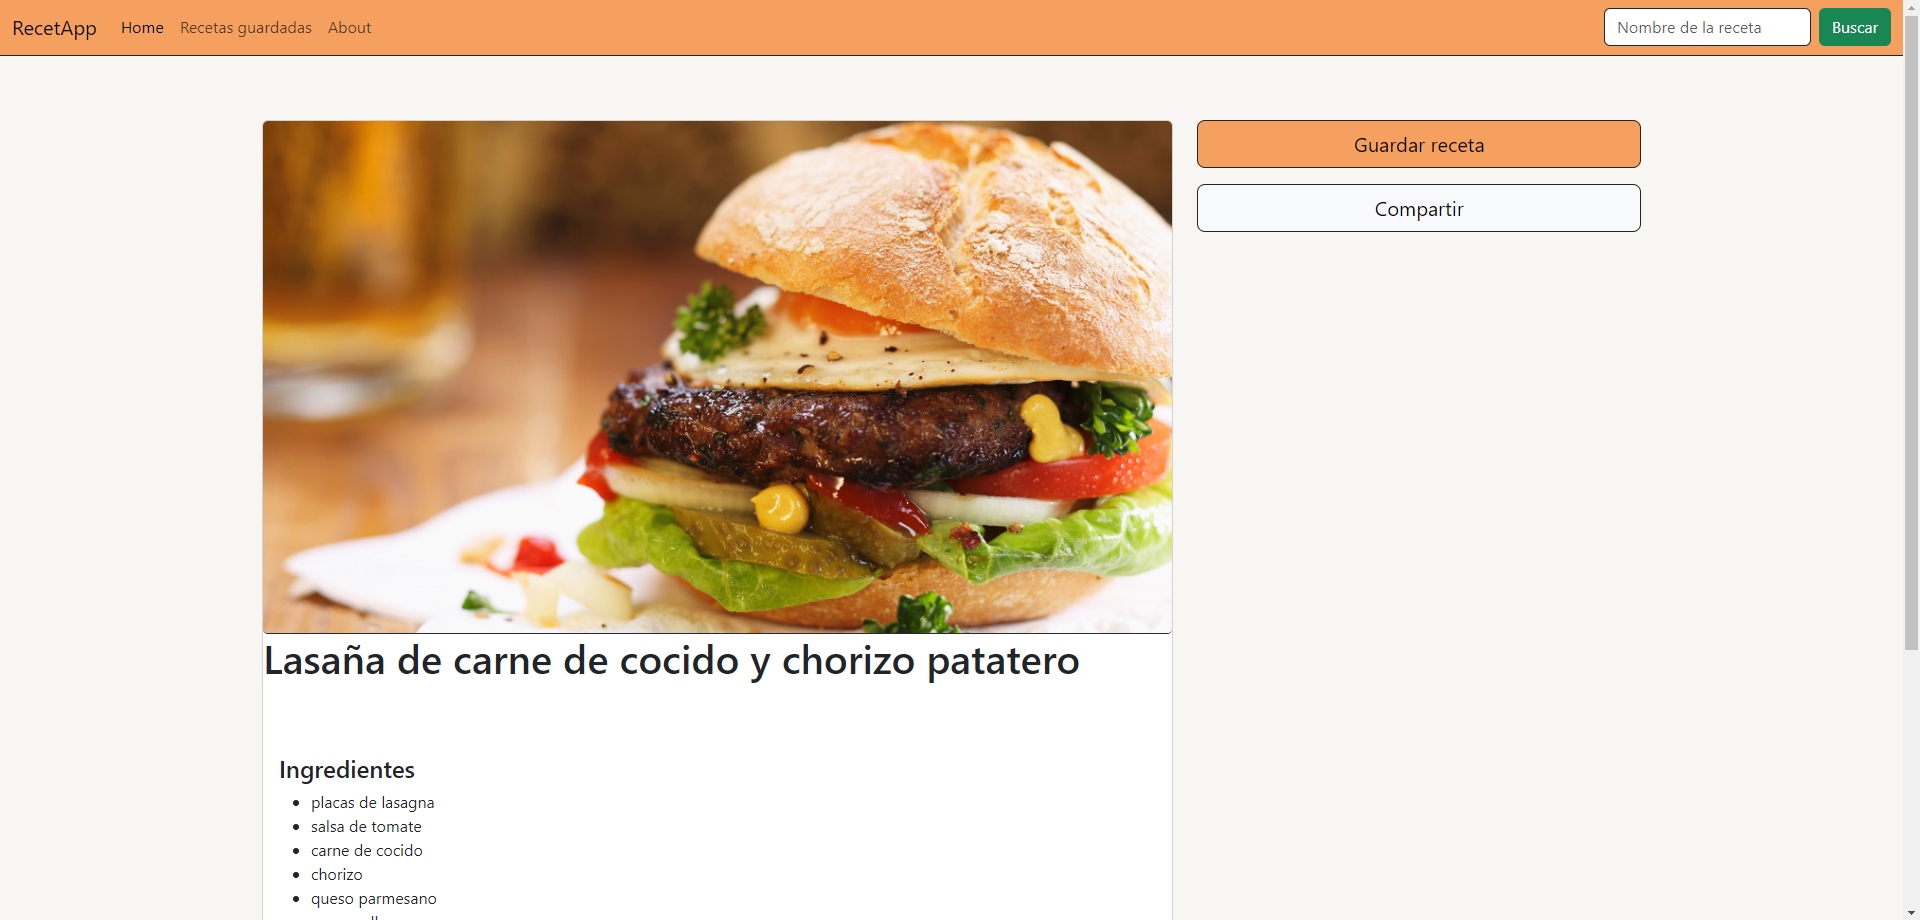
\includegraphics[width=120mm,scale=1]{./doc/imagenes/receta.png}}
\caption{Tarjeta de la receta ``Lasaña de carne''}
\label{fig:receta}
\end{figure}

\begin{figure}[h!]
\centering
\fbox{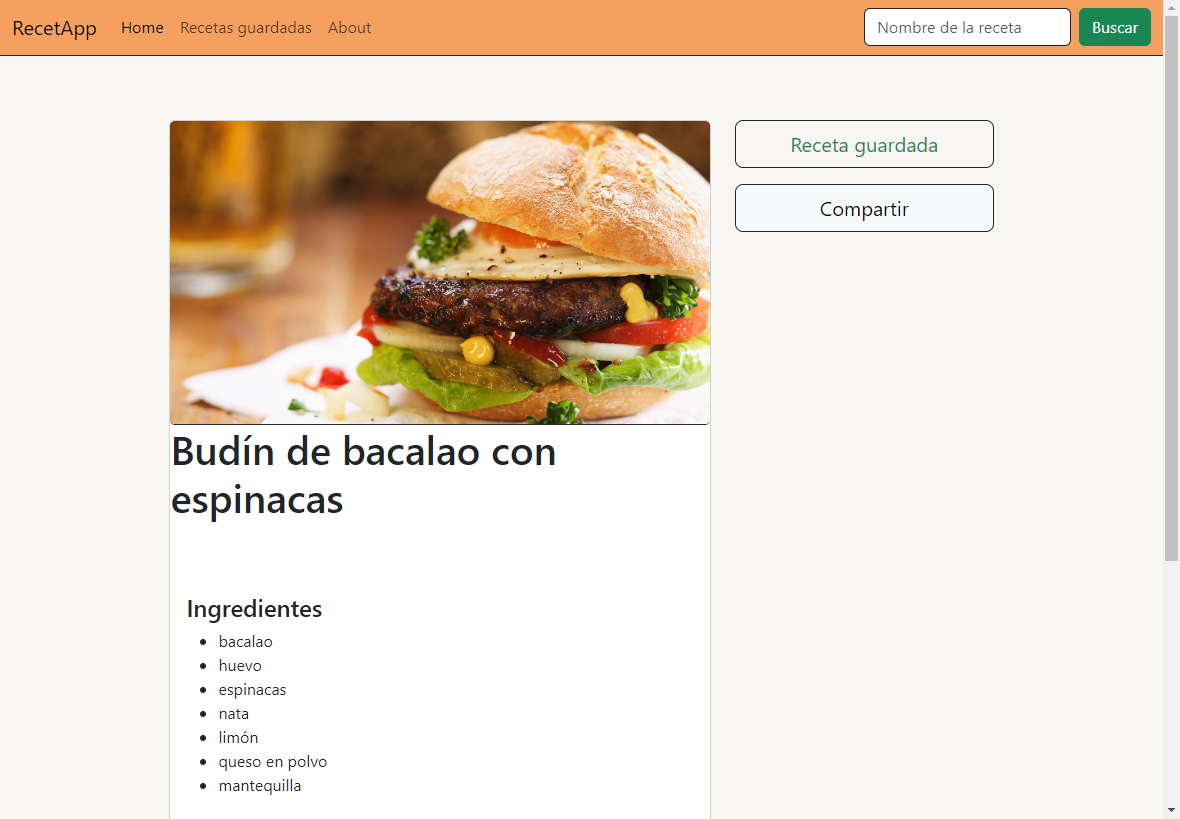
\includegraphics[width=100mm,scale=1]{./doc/imagenes/receta_ipad.png}}
\caption{Tarjeta de la receta ``Budín de bacalao'' en una tablet}
\label{fig:receta-tablet}
\end{figure}

\begin{figure}
\begin{lstlisting}[style=consola]
    <div class="row d-flex-inline bg-light rounded rounded-sm">
        <div class="col-lg-8">
            <div class="ms-5 mt-5 w-100">
                <h1>{{receta_nombre}}</h1>
                <div class="ms-2 ps-3 mt-5">
                    <h4>Ingredientes</h4>
                    <ul>
                    
                        <li>{{item}}</li>
                    
                    </ul>
                    <h4 class="mt-5">Pasos</h4>
                    <ol>
                        
                        <li>{{item}}</li>
                        
                    </ol>
                </div>
            </div>
        </div>
\end{lstlisting}
\caption{Código de la tarjeta de la receta}
\label{sni:}
\end{figure}

\newpage
\section{Framework}
Para pegar las dos capas desarrolladas hasta ahora: El núcleo para encontrar recetas y la capa de \gls{frontend}, se utiliza un \gls{framework} que actúa como intermediario estableciendo unos \gls{endpoint} para el usuario y algunas funcionalidades ya vistas en la sección anterior. 

Como ya se explicó en el apartado de implementación del proyecto, se ha elegido \Gls{django} como \gls{framework} para \Gls{python}. Este permite crear las rutas de manera sencilla y ofrece un modelo \gls{MVC} (Modelo-Vista-Controlador), que gestiona tanto la base de datos como la generación del \gls{HTML} que se ofrece al usuario. Además, permite crear plantillas \gls{HTML} dinámicas con los datos recuperados del modelo, y generar formularios que encajen con la generación de \glspl{tupla} para la \gls{base}. 

La instalación es muy sencilla, pudiéndose insertar en el entorno de \Gls{poetry} añadiendo las dependencias según lo explicado. \Gls{django} usa por defecto una \gls{base} SQLite 3 llamada ``db.sqlite3'' dentro del entorno de \Gls{django}, se puede cambiar el nombre mediante el parámetro \emph{DB\_Name} del fichero de configuración de entorno. Además es necesario añadir al software instalado el entorno de la nueva aplicación.

Iniciar una aplicación genera una platilla de ficheros de donde \Gls{django} obtendrá los datos para montar la lógica de la página web. 
\begin{figure}[h!]
\begin{lstlisting}[style=consola]
    poetry run django-admin startproject <nombre del proyecto>
    poetry run Python3 <carpeta del proyecto>/manage.py startapp <nombre de la aplicacion>
    invoke migrate --app=<nombre del proyecto>
\end{lstlisting}
\caption{Comandos para la instalación de Django}
\end{figure}

\newpage
\begin{figure}[h!]
    \dirtree{%
        .1 /.
        .2 app.
        .3 migrations.
        .3 static.
        .4 buscador.js.
        .3 templates.
        .4 base.html.
        .4 buscador.html.
        .4 receta.html.
        .4 resultados.html.
        .3 buscador.py.
        .3 configuration.py.
        .3 db.py.
        .3 urls.py
        .3 views.py
        .3 models.py
        .2 Dietplanner.
        .3 settings.py.
        .3 urls.py.   
        .2 Manage.py.
    }
    \caption{Estructura del proyecto}
    \label{fig:django}
\end{figure}
En la figura superior se muestra el árbol de directorios final que tiene el proyecto generado por \Gls{django}. En la carpeta ``app'' es donde se contiene toda la información de la aplicación. 

\subsection{Endpoints}
La definición de \gls{endpoint} tiene muchos significados diferentes dependiendo del contexto, en un entorno de programación el significado se refiere a una URL de una \gls{API} o \gls{backend} que se encarga de responder a una petición. 

Para el desarrollo del proyecto se han creado algunos \gls{endpoint} que sirven como punto de acceso a los datos de recetas almacenado en la base de datos. En \Gls{django} se definen en el archivo ``app/urls.py'', pero para que \Gls{django} pueda encontrarlos debemos incluir este fichero en las URL a nivel de proyecto, desde ``Dietplanner/urls.py''. 

\begin{figure}
    \centering
    \begin{lstlisting}[style=consola]
        urlpatterns = [
            path("", views.index, name="index"),
            path("buscar/", views.buscar, name="buscar_resultados"),
            path("resultados/", views.resultados, name="resultados"),
            path("receta/<int:id>", views.detalle_receta, name="detalle_receta")
        ]
    \end{lstlisting}
    \caption{Puntos de acceso de la aplicación}
    \label{sni:endpoints}
\end{figure}

\newpage
Dentro del fichero ``views.py'' se implementa la lógica de cada \gls{endpoint}. Se destacan los cuatro \glspl{endpoint} creados
\begin{itemize}
    \item índice
    \item Buscar
    \item Resultados
    \item Detalle receta
\end{itemize}

\subsubsection{Índice}
Este punto de acceso se utiliza por defecto al acceder a la página web inicialmente, y devuelve una vista de la plantilla ``buscador.html'' con el buscador principal y una columna de recetas aleatorias. 

\subsubsection{Buscar}
Anteriormente, en el apartado de interfaz, se explicó que el buscador de ingredientes principal, que se actualizaba la lista de ingredientes con cada letra que se introducía haciendo uso de un \gls{event}, dicha funcionalidad utiliza este \gls{endpoint}.

Al llegar una petición se comprueba el método, si viene de una solicitud ``GET'' se obtiene la cadena pasada como argumento. Posteriormente, por simplicidad, se utiliza un filtro en \Gls{django} para obtener todos los ingredientes que existen en la \gls{base}. 
\begin{figure}
    \centering
    \begin{lstlisting}[style=consola]
        resultados = buscador.buscarIngredientesNombre(query)
        for resultado in resultados:
            resultado_dict = {
                'id': resultado.id,
                'nombre': resultado.nombre,
            }
            resultados_lista.append(resultado_dict)
    \end{lstlisting}
    \caption{Endpoint buscar}
    \label{sni:Buscar}
\end{figure}
Para cada uno de los ingredientes encontrados como resultado se crea una cadena de texto en formato \gls{JSON} con toda la información relativa de los ingredientes, y en el lado de la \gls{interfaz} se gestionan los datos como se explicó anteriormente.

\subsubsection{Resultados}
Este \gls{endpoint} se especifica para obtener los resultados de las recetas que puede hacer el usuario con los ingredientes que desea utilizar en la cocina. En la aplicación existen dos tipos de búsqueda de recetas
\begin{itemize}
    \item Ingredientes
    \item Nombres
\end{itemize}

Dependiendo del tipo de búsqueda se añade un parámetro que lo especifica. En caso de buscar por ingredientes, se obtienen de la \gls{cookie} guardada en el navegador, convertida a una lista de enteros que se pasa como argumento a la función \textit{buscarRecetasIngredientes} del buscador, explicada en capítulos anteriores.

Esta devuelve la lista de recetas que se pasa como contexto al \gls{render} de la plantilla \gls{HTML}, para darle el formato final. 

\subsubsection{Detalle receta}
Este \gls{endpoint} recibe como argumento el identificador de la receta a la que se está intentando acceder. 

Se obtiene la receta haciendo uso del método \emph{buscarRecetasID} de la clase \emph{Buscador}. Posteriormente, se les da el formato a los pasos de la receta para listarlos de manera sencilla, por último, se añade la información al contexto que se pasa al \gls{render}.